\documentclass{article}
\usepackage{femape}
\usepackage{graphicx}
\usepackage{stmaryrd}
\title{Grundlagen der Logik}
\author{Felix Leitl}
\begin{document}
	\maketitle
	\newpage
	\section{Aussagenlogische Konsequenz und Beweise}
		\subsection{Wahrheitstafel}
			\begin{center}
				\begin{tabular}{c|c|c|c|c}
					A & B & C & A \to B & ...\\
					\hline
					w & w & w & w & ...\\
					\hline
					w & w & f & w & ...\\
					\hline
					w & f & w & f & ...\\
					\hline
					w & f & f & f & ...\\
					\hline
					f & w & w & w & ...\\ 
					\hline
					f & w & f & w & ...\\
					\hline
					f & f & w & w & ...\\
					\hline
					f & f & f & w & ...
				\end{tabular}
			\end{center}
		Formel ist eine aussagenlogische Konsequenz, wenn beide Spalten übereinstimmen
		\subsection{Coq}
			\begin{center}
				\begin{tabular} {c|c|c|c}
					$\land I$ & split. &  \\
					\hline
					$\land E_1$ & destruct H as [H0 \_]; exact H0. &  \\
					\hline
					$\land E_2$ & destruct H as [\_ H0]; exact H0. &  \\
					\hline
					$\lor I_1$ & left. &  \\
					\hline
					$\lor I_2$ & right. &  \\
					\hline
					$\lor E$ & destruct H as [L|R]. apply H0; exact L. apply H1; exact R. \\
					\hline
					$\to I$ & intro. & $A \to B$ & $A \quad B$ \\
					\hline
					$\to E$ & apply H; exact H0. &  \\
					\hline
					$\lnot I$ & intro. & & $\lnot A \quad \bot$ \\ 
					\hline
					$\lnot E$ & apply NNPP. & $\lnot\lnot A$ & $A$ \\
					\hline
					$\bot I$ & apply H & & \\
					\hline
					$\bot E$ & contradiction & & \\
					\hline
					& assert ($\lnot$ A) &  neu UZ -> alt An 
				\end{tabular}
			\end{center}
	\section{Formalisierung in Prädikatenlogik}
	\section{Unifikation}
		\subsection{Regeln} % I hope this is correct
			\begin{center}
				\begin{tabular} {c|c|c}
					Regel & Pre & After \\
					\hline
					decomp & $f(x)=f(y)$ & $x=y$ \\
					\hline
					delete & $f(x) = f(x)$ & \\
					\hline
					orient & $f(x) = y$ & $y = f(x)$ \\
					\hline
					elim & $f(x) = y \quad x = z$ & $f(z)= y \quad x = z$ \\
					\hline
					conflict & $f(x) = g(x)$ & \bot \\
					\hline
					occur & $f(x) = x $ & \bot
				\end{tabular}
			\end{center}
		\subsection{Algorithm}
			Die Formel ist syntaktisch identisch, hat also einen most generic unifier (mgu), wenn der Algorithmus endet, ohne \bot. \newline
			Bsp.: $x=h(h(w)) \quad z = h(w) \quad \Rarr \quad mgu = [\frac{h(h(w))}{x}, \frac{h(w)}{z}]$
	\section{Prädikatenlogische Resolution}
		\subsection{Kodierung von $\to$ durch $\lnot$ und $\lor$}
			$A\to B \equiv \lnot A \lor B$
		\subsection{Negationsnormalform}
			$\lnot$ an innerste Stelle ziehen: \newline
			$\forall y.\lnot(\lnot y \land \exists x. R(x))\equiv \forall y.y \lor \forall x \lnot R(x)$ \newline
			Aus $\land$ wird $\lor$, aus $\forall$ wir $\exists$ und umgekehrt. 
		\subsection{Pränexe Normalform}
			Alle Quantoren nach vorne ziehen, bei Variablendopplung neue Variablen einführen
		\subsection{Skolemform}
			Nicht allquantorifizierte Variablen mittels Substitution durch Funktionen austauschen 
			$\sigma[\frac{f(x)}{x}, \frac{h(x)}{y}]$
		\subsection{Konjunktive Normalform (KNF)}
			$(A\lor B)\land (C \lor A)$	
		\subsection{Klauselform}
			Klauseln entlang der KNF Konjunktionen brechen \newline
			$\{A, B\}\{C, A\}$
		\subsection{Unerfüllbarkeit durch Klauselmenge zeigen}
			Idee: wenn man die leere Menge herleiten kann, dann ist die Formel unerfüllbar. \newline
			Je zwei widersprüchliche Aussagen auslöschen und den Rest der zwei Klauseln zu einer neuen verschmelzen. Mittels Substitution Widersprüche aufzeigen. \newline
			%Nachfolgende wahrscheinlich großer Blödsinn
			Bei Beweis für Erfüllbarkeit, Klauselmenge um flache Aussage erweitern, wenn dann nicht erfüllbar, dann ist die Ursprungsformel erfüllbar
	\section{Formale Deduktion}
		\subsection{Fitch}
			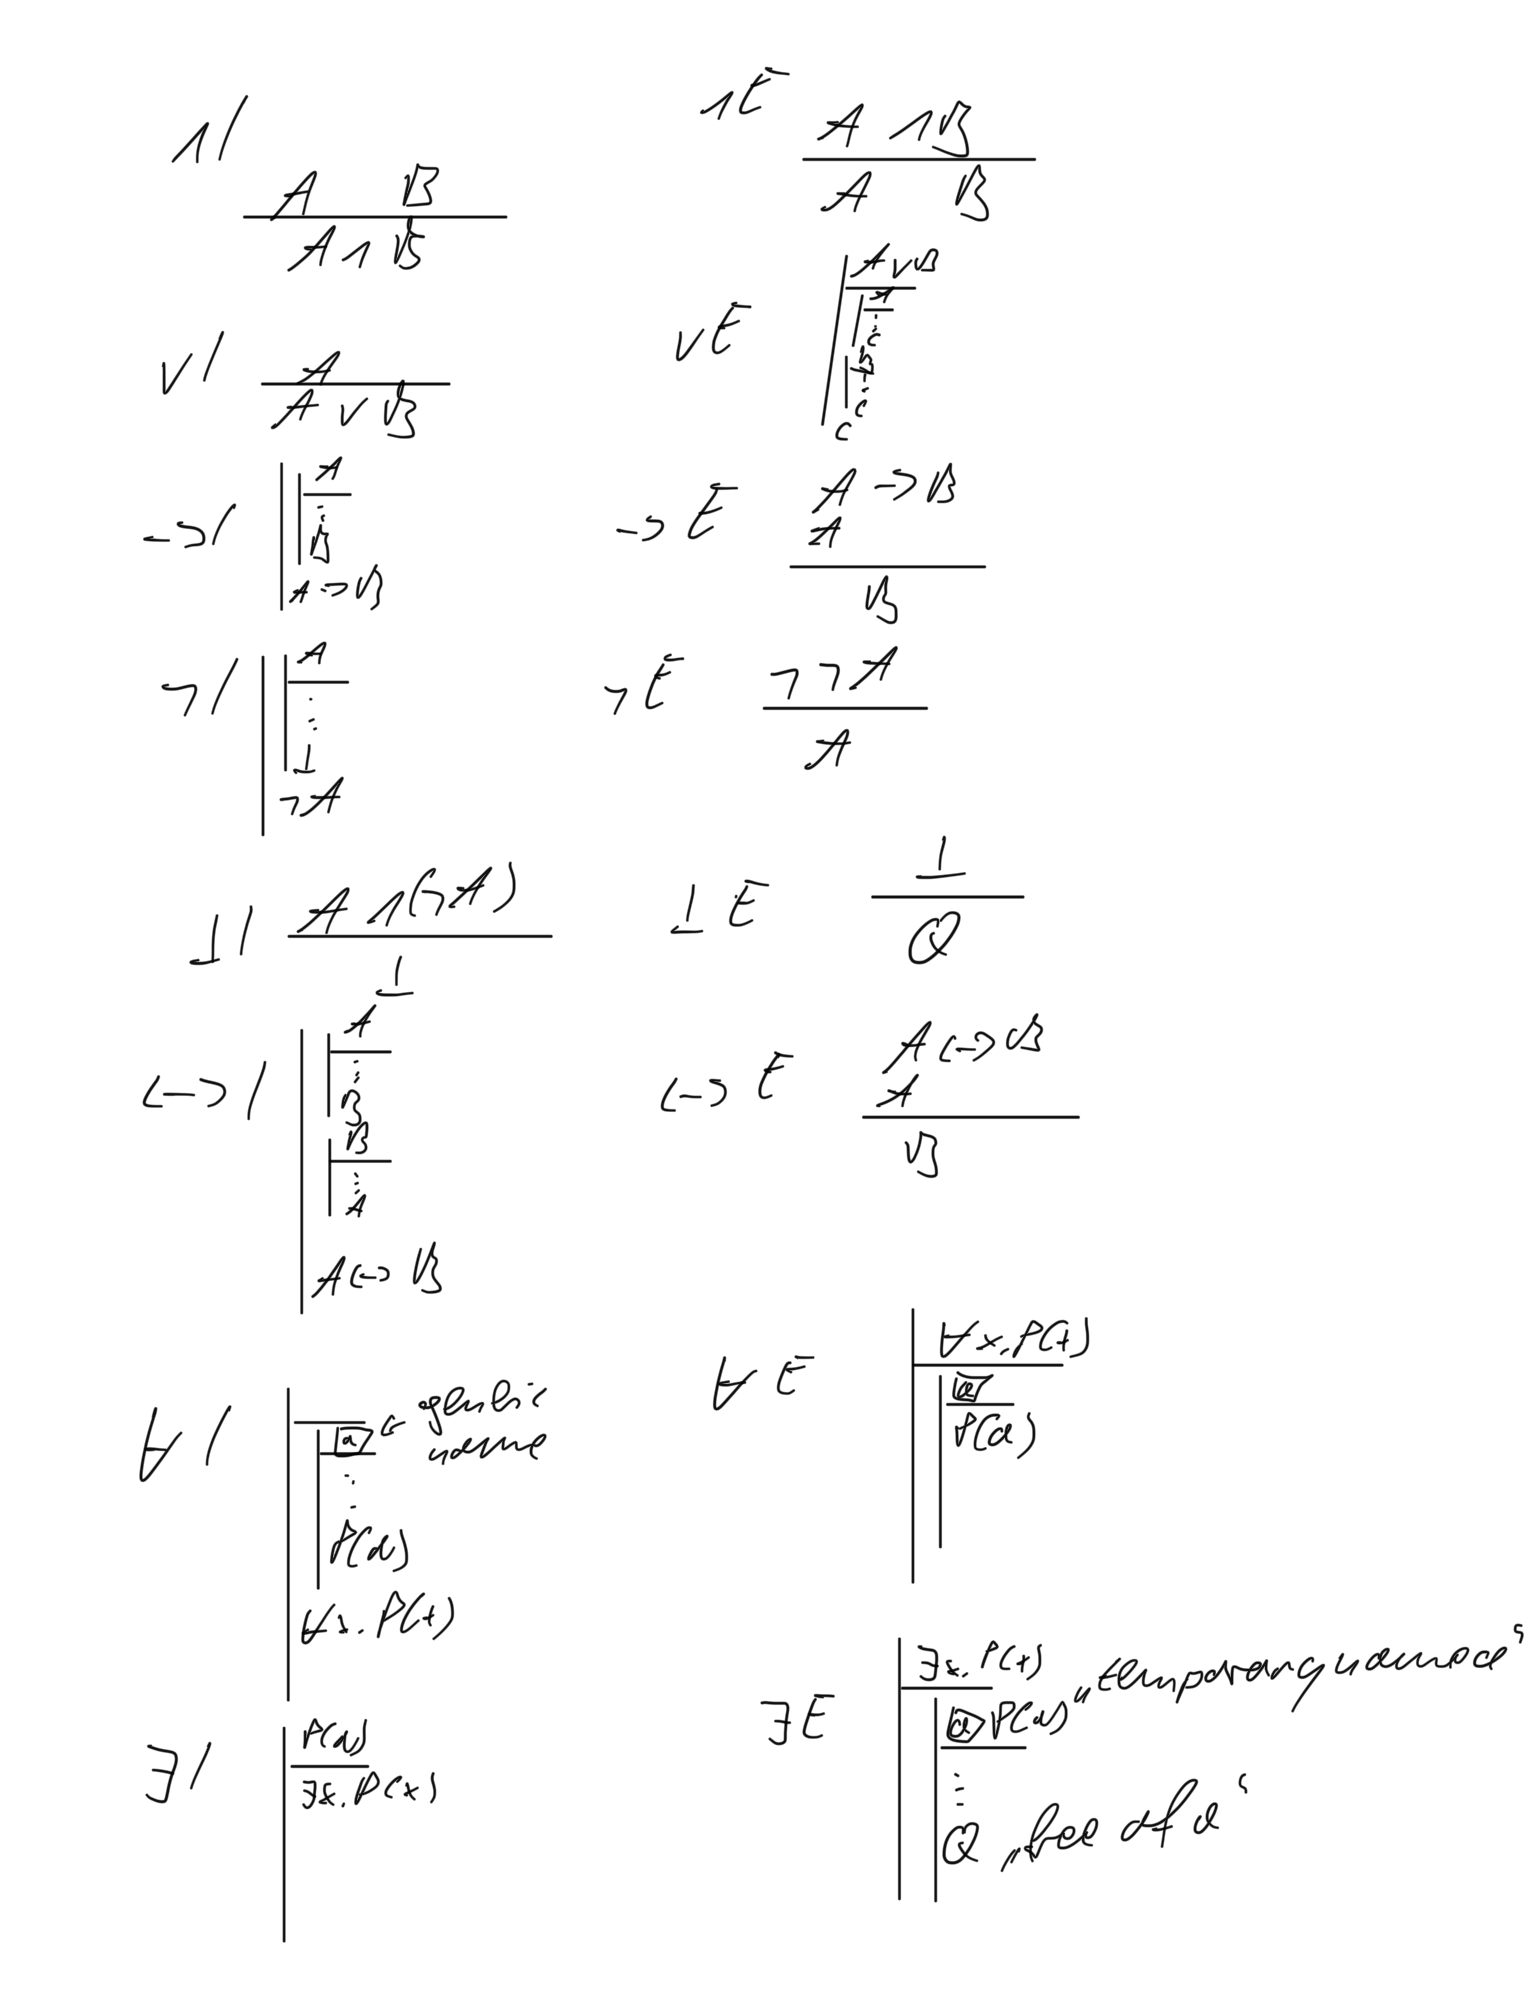
\includegraphics[scale=0.3]{IMG_0800.PNG}
	\section{Induktion}
		Geschlossene $\Sigma$-Terme werden durch die Grammatik $E::=zero/one/mult(E_1,E_2)$ dargestellt \newline
		Induktion über $E$:
			\begin{itemize}
				\item $E=zero:\frak{m}\llbracket zero\rrbracket=0\in\{0, 1\}$
				\item $E=one:\frak{m}\llbracket one\rrbracket=1\in\{0, 1\}$
				\item $E=mult(E_1, E_2):$ Nach IV wissen wir $\frak{m}\llbracket E_1\rrbracket\in\{0, 1\}$ und $\frak{m}\llbracket E_2\rrbracket\in\{0, 1\}$ \newline
					$\frak{m}\llbracket E\rrbracket=\frak{m}\llbracket mult(E_1, E_2)\rrbracket=\frak{m}\llbracket mult\rrbracket(\frak{m}\llbracket E_1\rrbracket, \frak{m}\llbracket E_2\rrbracket) = \frak{m}\llbracket E_1\rrbracket \cdot \frak{m}\llbracket E_2\rrbracket$	
			\end{itemize}
		Es ergeben sich 4 Fälle:
			\begin{itemize}
				\item $0 \cdot 0$
				\item $0 \cdot 1$
				\item $1 \cdot 0$
				\item $1 \cdot 1$
			\end{itemize}
		$\Rarr$ $\frak{m}\llbracket E\rrbracket\in\{0, 1\}$ in allen Fällen
		$\dreieck$

\end{document}









